\documentclass[12pt]{article}
\usepackage[margin=1in]{geometry}
\usepackage{graphicx}
\usepackage{xcolor}
\usepackage{amsmath}
\usepackage{amsfonts}
\usepackage{amssymb}
\usepackage{cleveref}
\usepackage{subfigure}
\usepackage{lineno}
\usepackage{setspace}

\newcommand{\hl}[1]{\colorbox{yellow}{#1}}

\newcommand{\vA}{\mathbf{A}}
\newcommand{\vB}{\mathbf{B}}
\newcommand{\vBi}{\mathbf{B}^{(i)}}
\newcommand{\vBj}{\mathbf{B}^{(j)}}
\newcommand{\vC}{\mathbf{C}}
\newcommand{\vu}{\mathbf{u}}
\newcommand{\bw}{\mathbf{w}}
\newcommand{\vw}{\mathbf{w}}
\newcommand{\bv}{\mathbf{v}}
\newcommand{\vv}{\mathbf{v}}
\newcommand{\cN}{\mathcal{N}}
\newcommand{\cI}{\mathcal{I}}
\newcommand{\vr}{\mathbf{r}}
\newcommand{\cQnet}{\mathcal{Q}_{\text{net}}}
\newcommand{\cP}{\mathcal{P}}
\newcommand{\bk}{\mathbf{k}}
\newcommand{\cQ}{\mathcal{Q}}
\newcommand{\vP}{\mathbf{P}}
\newcommand{\bvC}{\bar{\mathbf{C}}}
\newcommand{\bvA}{\bar{\mathbf{A}}}
\newcommand{\bvB}{\bar{\mathbf{B}}}
\newcommand{\vW}{\mathbf{W}}
\newcommand{\vPhi}{\boldsymbol{\Phi}}
\newcommand{\vPhiplus}{\boldsymbol{\Phi}^{+}}
\newcommand{\bu}{\bar{u}}
\newcommand{\bepsilon}{\boldsymbol{\epsilon}}
\newcommand{\bsigma}{\boldsymbol{\sigma}}
\newcommand{\phii}{\phi^{(i)}}
\newcommand{\vI}{\mathbf{I}}
\newcommand{\vzero}{\boldsymbol{0}}
\newcommand{\vz}{\mathbf{z}}
\newcommand{\vM}{\mathbf{M}}
\newcommand{\vg}{\mathbf{g}}
\newcommand{\phij}{\phi^{(j)}}
\newcommand{\Ti}{T^{(i)}}
\newcommand{\Tj}{T^{(j)}}
\newcommand{\ui}{u^{(i)}}
\newcommand{\vH}{\mathbf{H}}
\newcommand{\uj}{u^{(j)}}
\newcommand{\vF}{\mathbf{F}}
\newcommand{\vui}{\mathbf{u}^{(i)}}
\newcommand{\vuj}{\mathbf{u}^{(j)}}
\newcommand{\cV}{\mathcal{V}}
\newcommand{\vTheta}{\boldsymbol{\Theta}}
\newcommand{\bvf}{\bar{\mathbf{f}}}
\newcommand{\vphi}{\boldsymbol{\phi}}
\newcommand{\vvarphi}{\boldsymbol{\varphi}}
\newcommand{\deltavu}{\delta\mathbf{u}}
\newcommand{\vvarphiij}{\boldsymbol{\varphi}_{i}^{j}}
\newcommand{\vvarphiijT}{\boldsymbol{\varphi}_{i}^{j\top}}
\newcommand{\vD}{\mathbf{D}}
\newcommand{\vf}{\mathbf{f}}
\newcommand{\vfBC}{\mathbf{f}_{\text{BC}}}
\newcommand{\vAi}{\mathbf{A}^{(i)}}
\newcommand{\vCi}{\mathbf{C}^{(i)}}
\newcommand{\vfQ}{\mathbf{f}_{\mathcal{Q}}}
\newcommand{\bvu}{\bar{\mathbf{u}}}
\newcommand{\phik}{\phi_k}
\newcommand{\phil}{\phi_l}
\newcommand{\Ei}{E^{(i)}}
\newcommand{\dirichletset}{\left\{T_b\right\}}
\newcommand{\eij}{e_{ij}}
\newcommand{\jump}[1]{\left[#1\right]}
\newcommand{\average}[1]{\left\{#1\right\}}
\newcommand{\sumneighbori}{\sum_{j\in\mathcal{N}_i}}
\newcommand{\sumneighborj}{\sum_{i\in\mathcal{N}_j}}
\newcommand{\sumneighbordirichlet}{\sum_{j\in\mathcal{N}_i\cup\left\{T_b\right\}}}
\newcommand{\eiq}{e_{iq}}
\newcommand{\eiT}{e_{iT}}
\newcommand{\intEi}{\int_{E^{(i)}}}
\newcommand{\barui}{\bar{u}^{(i)}}
\newcommand{\baruj}{\bar{u}^{(j)}}
\newcommand{\Rij}{R_{ij}}
\newcommand{\cE}{\mathcal{E}}
\newcommand{\cG}{\mathcal{G}}
\newcommand{\vBiij}{\mathbf{B}^{(i)}_{ij}}
\newcommand{\vBjij}{\mathbf{B}^{(j)}_{ij}}
\newcommand{\vfi}{\mathbf{f}^{(i)}}
\newcommand{\vK}{\mathbf{K}}
\newcommand{\tvK}{\tilde{\mathbf{K}}}
\newcommand{\tk}{\tilde{k}}
\newcommand{\cK}{\mathcal{K}}
\newcommand{\vk}{\boldsymbol{k}}
\newcommand{\tcK}{\tilde{\mathcal{K}}}
\newcommand{\tvk}{\tilde{\boldsymbol{k}}}
\newcommand{\tvkappa}{\tilde{\boldsymbol{\kappa}}}
\newcommand{\vkappa}{\boldsymbol{\kappa}}
\newcommand{\vp}{\mathbf{p}}
\newcommand{\vd}{\mathbf{d}}
\newcommand{\vq}{\mathbf{q}}
\newcommand{\vLambda}{\boldsymbol{\Lambda}}
\newcommand{\vG}{\mathbf{G}}
\newcommand{\vR}{\mathbf{R}}
\newcommand{\vbeta}{\boldsymbol{\beta}}
\newcommand{\vQ}{\mathbf{Q}}
\newcommand{\vO}{\mathbf{O}}
\newcommand{\vy}{\mathbf{y}}
\newcommand{\vE}{\mathbf{E}}

% graphics
\newcommand\insertfigs[3]{
\subfigure[\label{#1}#3]{\includegraphics[width=#2\linewidth]{#1}}
}

% d#/dt
\newcommand{\ddt}[1]{\frac{\dd #1}{\dd t}}
\newcommand{\ddtb}[1]{\frac{\dd^2#1}{\dd t^2}}
\newcommand{\ddtn}[2]{\frac{\dd^#2#1}{\dd t^#2}}
% p#/pt
\newcommand{\ppt}[1]{\frac{\partial#1}{\partial t}}
\newcommand{\pptb}[1]{\frac{\partial^2#1}{\partial t^2}}
\newcommand{\pptn}[2]{\frac{\partial^#2#1}{\partial t^#2}}

\newcommand\vn{{\mathbf{n}}}

\begin{document}
\onehalfspacing
\linenumbers

\title{Physics-Infused Reduced-Order Modeling for Analysis of Ablating Hypersonic Thermal Protection Systems}

\maketitle

\begin{abstract}
    This work presents a physics-infused reduced-order modeling (PIROM) framework towards the design, analysis, and optimization of non-decomposing ablating hypersonic thermal protection systems (TPS). 
\end{abstract}

\section{Introduction}


\section{Modeling of Ablating Thermal Protection Systems}

This section presents the ablation problem for a non-decomposing TPS as a parametrized system of non-linear PDEs. These non-linear PDEs govern the energy of heat conduction and the pseudo-elastic material deformation of the mesh motion. Two different but mathematically-connected numerical solution strategies are provided: (1) a high-fidelity full-order model (FOM) based on a discontinuous Galerkin FEM, and (2) a thermo-elastic RPM based on a one-dimensional approximation to the energy and pseudo-elasticity equations.

\subsection{Governing Equations}\label{sec_governing_equations}

Consider a generic domain $\Omega\subset$, $d=2$ or $3$, illustrated in Fig.~\ref{fig_general_domain}. A heat flux $q_b(x,t)$ is prescribed on the boundary $\Gamma_q$ (i.e., Neumann boundary condition), and the temperature $T_b(x,t)$ is prescribed on boundary $\Gamma_T$ (i.e., Dirichlet boundary condition), where $\Gamma_q\cup\Gamma_T = \partial\Omega$ and $\Gamma_q\cap\Gamma_T = \emptyset$. The ablation occurs only on the heated boundary $\Gamma_q$, and its effects are included into the energy equation using an Arbitrary Lagrangian-Eulerian (ALE) description. The ALE assumes that the displacement $\vw(x,t)\in\mathbb{R}^d$ of the computational mesh moves with velocity $\vv(x,t)$ that is different to the material velocity, which is fixed to zero in this work.

\begin{figure}
    \centering
    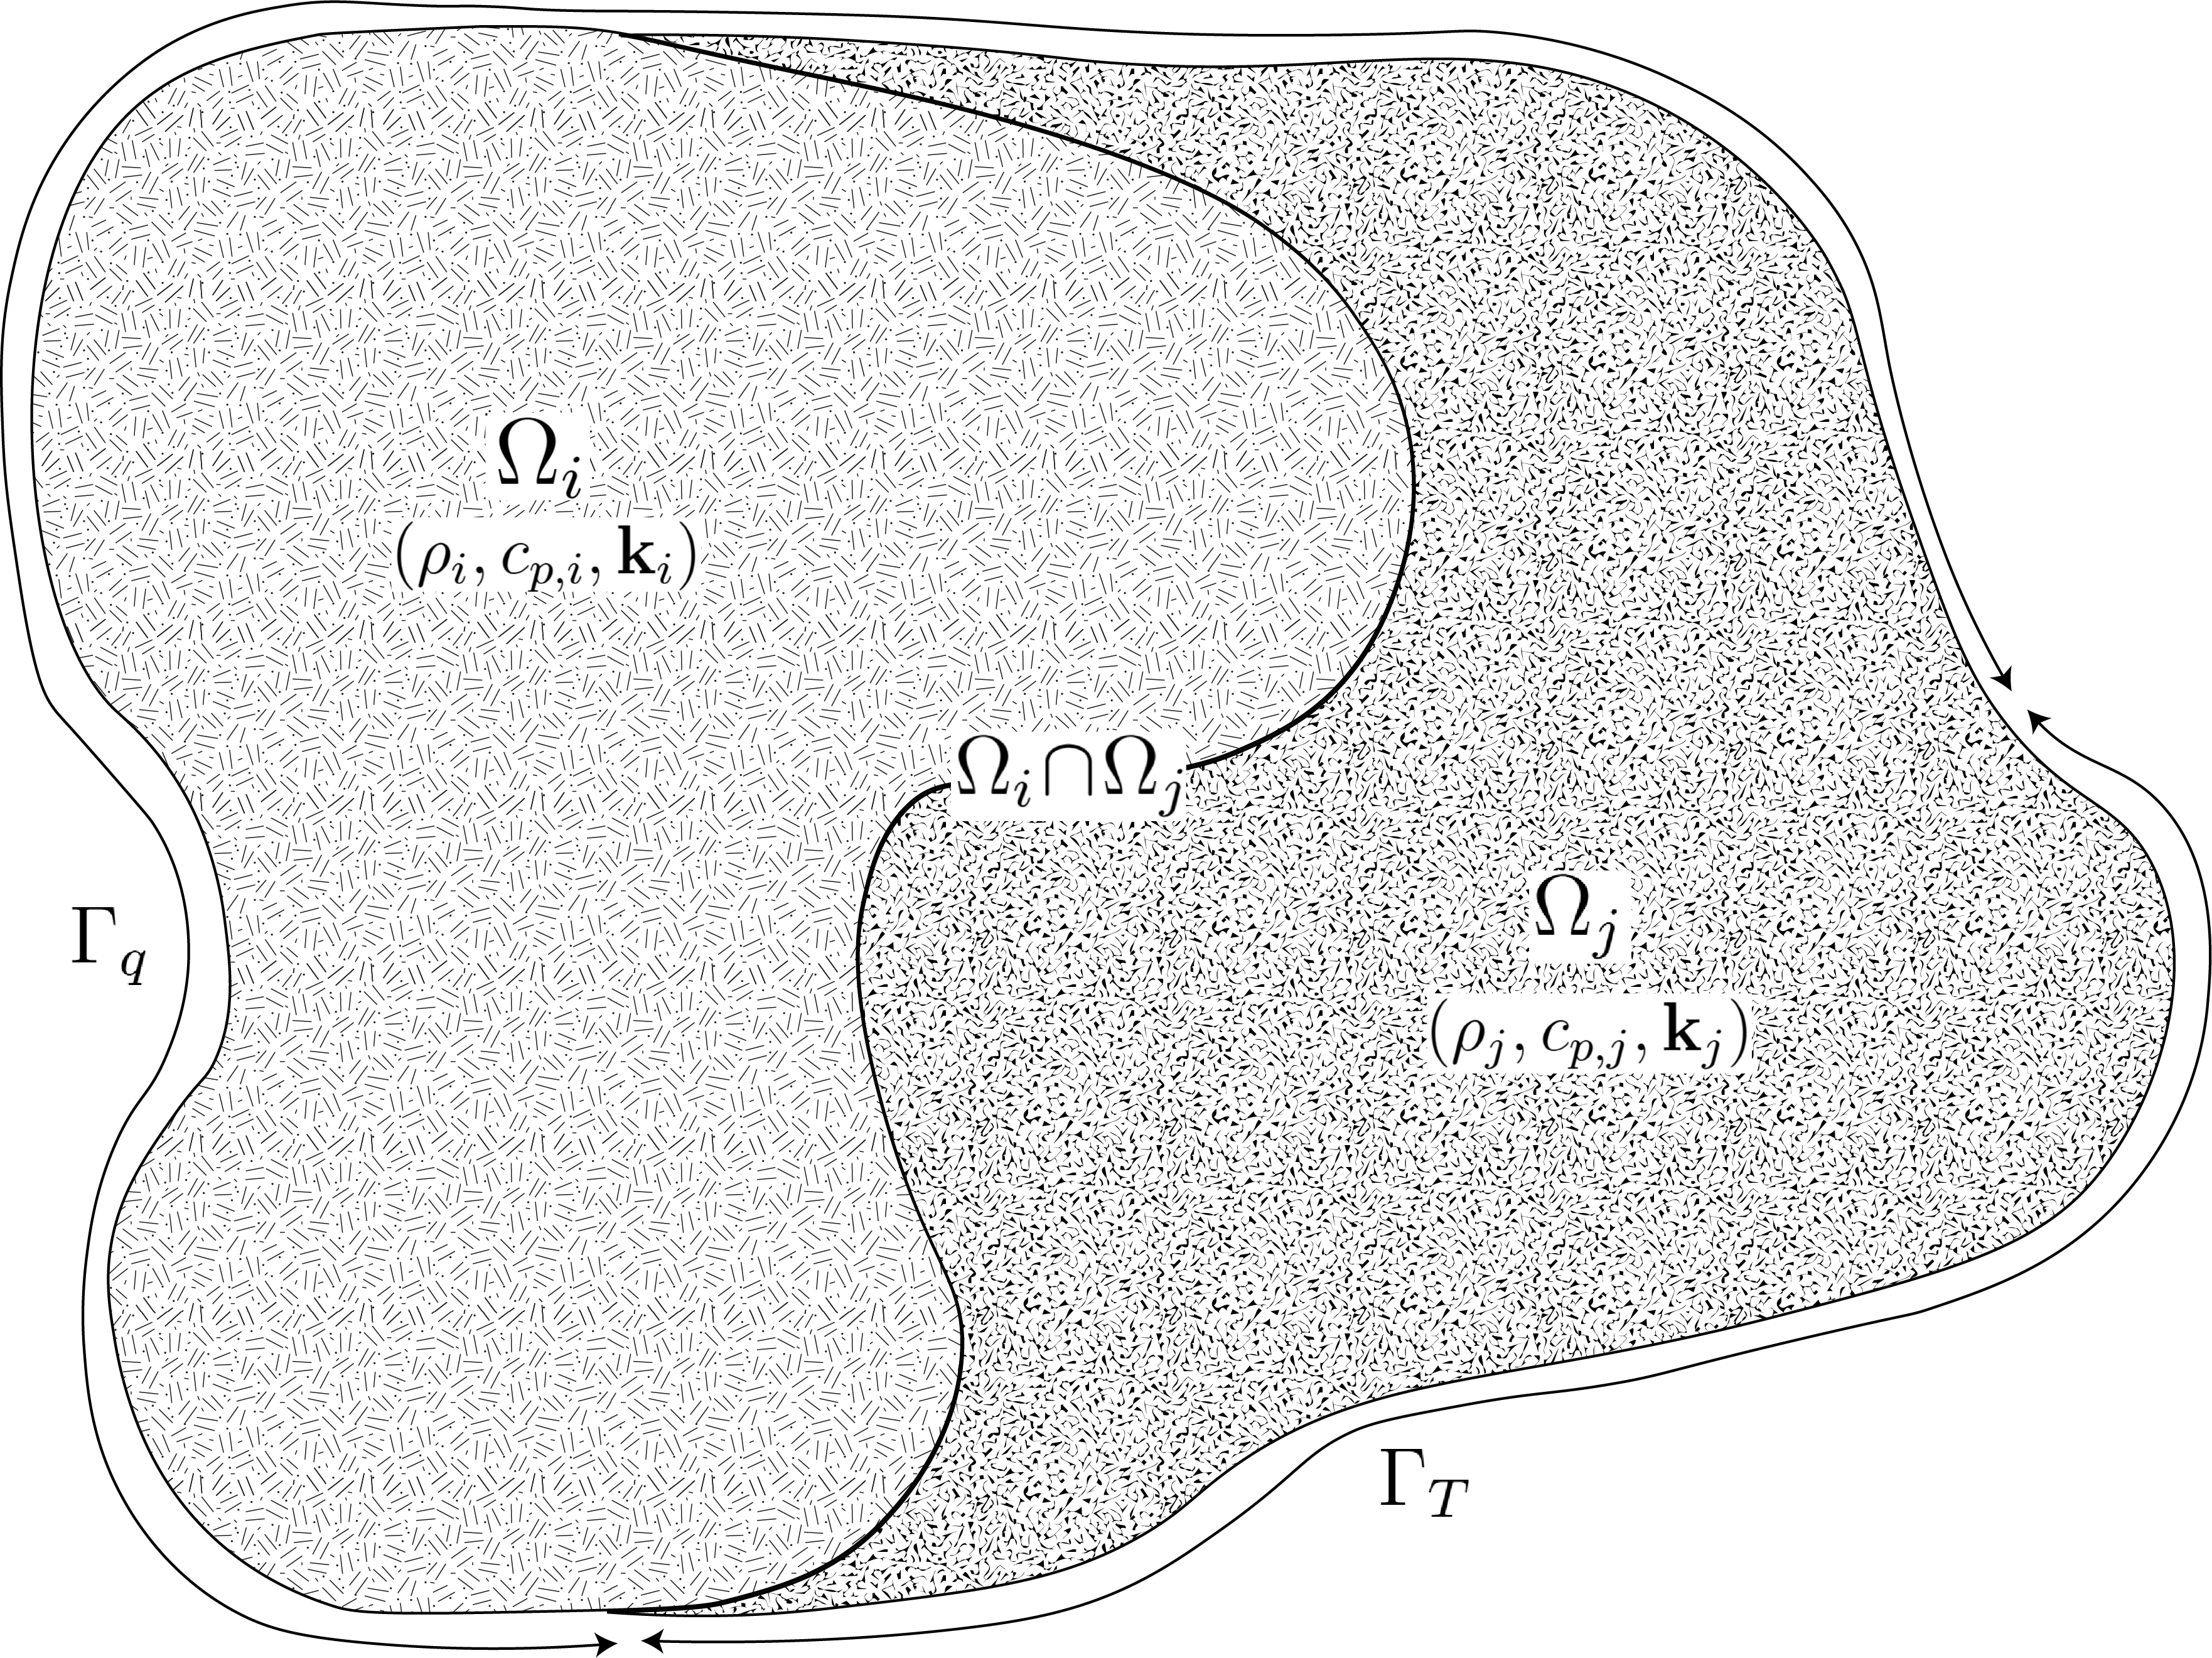
\includegraphics[width=0.6\textwidth]{./figs/general_domain.png}
    \caption{General domain $\Omega$ with prescribed heat flux $q_b(x,t)$ and temperature $T_b(x,t)$ on the boundaries $\Gamma_q$ and $\Gamma_T$, respectively. The mesh moves with a velocity $\mathbf{v}(x,t)$, while the material velocity is $\mathbf{w}(x,t)$.\hl{draw mesh next to arbitrary domain with moving boundaries.}}
    \label{fig_general_domain}
\end{figure}

The transient heat conduction is described by the energy equation,
\begin{subequations}
    \begin{align}
        \rho c_p\left(\ppt{T} - \mathbf{v}(x,t)\cdot\nabla T\right) - \nabla\cdot (\mathbf{k}\nabla T) &= \cQ(x,t),\ x\in\Omega \label{eqn_thermal_pde}\\
        -\mathbf{k}\nabla T\cdot \vn &= q_b(x,t),\ x\in\Gamma_q\label{eqn_thermal_bc_neumann}\\
        T(x,t) &= T_b(x,t),\ x\in\Gamma_T\label{eqn_thermal_bc_dirichlet}\\
        T(x,0) &= T_0(x),\ x\in\Omega\label{eqn_thermal_ic}
    \end{align}\label{eqn_governing_equations}
\end{subequations}
while the mesh motion is described by the pseudo-elasticity equation,
\begin{subequations}
    \begin{align}
        \nabla\cdot\boldsymbol{\sigma}(\mathbf{w}) &= 0\label{eqn_elasticity_pde}\\
        \vw(x,t) &= \vw_q(x,t),\quad x\in\Gamma_q\label{eqn_displacement_heated_bc}\\
        \vw(x,t) &= 0,\quad x\notin \Gamma_q\label{eqn_displacement_unheated_bc}\\
        \vw(x,0) &= \boldsymbol{0}\label{eqn_displacement_initial_condition}
    \end{align}
\end{subequations}

The density $\rho$, heat capacity $c_p$, and thermal conductivity $\mathbf{k}\in\mathbb{R}^{n_d\times n_d}$ are assumed to be constant with respect to temperature in this work. The terms in \cref{eqn_thermal_pde}, in the order they appear, correspond to the unsteady energy storage, heat conduction, temperature advection due to mesh motion, and the heat source terms. 

The elasticity equation \cref{eqn_elasticity_pde} states that the divergence of the stress tensor $\boldsymbol{\sigma}(\mathbf{w})$ is zero. The stress tensor is related to the strain tensor $\bepsilon(\bw)$ through Hooke's law,
\[
    \boldsymbol{\sigma}(\bw) = \mathbb{D}:\boldsymbol{\epsilon}(\bw)
\]
where $\mathbb{D}$ is the constitutive operator, ``:'' is the double contraction of tensors, and $\bepsilon$ is the symmetric strain tensor given by,
\[
    \bepsilon(\bw) = \frac{1}{2}\left(\nabla\bw + \nabla\bw^T\right)
\]
For instance, an isotropic material assumption results in,
\[
    \bsigma = \lambda\left(\nabla\cdot\bw\right) \mathbf{I} + 2\mu\bepsilon(\bw)
\]
where $\lambda$ and $\mu$ are Lame constants that are arbitrarily selected to model the mesh motion. The ``material'' properties $\lambda$ and $\mu$ can be chosen to tailor the mesh deformation and need not represent the actual material being modeled~\hl{Amar2016}. 

The boundary conditions for the energy equation includes a heated surface (\cref{eqn_thermal_bc_neumann}) and a constant-temperature surface (\cref{eqn_thermal_bc_dirichlet}). The boundary conditions for the pseudo-elasticity equation are a function of the surface temperature $T_q(x,t)$ for $x\in\Gamma_q$ using a B' table. The B' table....
\begin{equation}
    \bw_q(x,t) = \int_{0}^{t} \mathbf{v}(x,\tau)d\tau = \int_{0}^{t}\mathbf{f}\left(T_q(x,\tau)\right)d\tau\label{eqn_boundary_displacement}
\end{equation}


\subsection{Full-Order Model: Finite-Element Method}\label{sec_fom}

To obtain the full-order numerical solution, the governing equation is spatially discretized using the variational principle from Discontinuous Galerking (DG) to result in a high-dimensional system of ODEs for the time-varying nodal data. The full-order TPS ablation simulations are computed using standard FEM instead, and the equivalence between DG and standard FEM is noted upon their convergence.

Consider a conforming mesh partition domain, where each element belongs to one and only one component. Denote the collection of all $M$ elements as $\left\{E_i\right\}_{i=1}^{M}$. In an element $E_i$, its shared boundaries with another element $E_j$, Neumann BC, and Dirichlet BC are denoted as $e_{ij}$, $e_{iq}$, and $e_{iT}$, respectively. Lastly, $\left|e\right|$ denotes the length $(n_d=2)$ or area $(n_d=3)$ of a component boundary $e$.

For the $i$-th element, use a set of $n^{(i)}$ trial functions, such as polynomials, to represent the temperature distribution,
\begin{equation}
    T^{(i)}(x,t) = \sum_{i=1}^{n^{(i)}} \phi_i^{(i)}(x)u_i^{(i)} \equiv \boldsymbol{\phi}^{(i)}(x)^T\vu^{(i)}(t)\label{eqn_element_temperature}
\end{equation}


By standard variational processes, e.g., \hl{Cohen2018}, the full governing equation is denoted as,
\begin{equation}
    \vA(\vu)\dot{\vu} = \left(\vB(\vu) + \vC(t)\right)\vu + \mathbf{f}(t)\label{eqn_energy_fem}
\end{equation}
where $\vu = \left(\vu^{(1)}, \vu^{(2)}, \ldots, \vu^{(M)}\right)^T\in\mathbb{R}^{MP}$ includes all the DG variables, $\mathbf{f}\in\mathbb{R}^{MP}$ is the external forcing, and the system matrices $\vA$, $\vB$, and $\vC$ are due to heat capacity, heat conduction, and temperature advection, respectively. The detailed formulation of the DG model is provided in Appendix~\hl{DG-FEM}.

\subsection{Reduced-Physics Model: Lumped-Capacitance Model}

This section presents the main results regarding the derivation of the LCM for ablating materials, and the main details are provided in Appendix~\hl{x}. The RPM is based on a coarse-grained temperature approximation in each component, neglecting higher-order spatial information that is critical to predict surface temperatures and thus the rate of surface recession. 

\subsubsection{Finite-Element Method and Component Interactions}

The arbitrary domain in Fig.~\ref{fig_general_domain} is partitioned into $N$ components $\left\{\Omega^{(i)}\right\}_{i=1}^{N}$, each with $\left\{E^{(i)}_j\right\}_{j=1}^{n^{(i)}}$ finite elements, establishing the resolution for the temperature and mesh displacement fields over each component. Figure~\hl{x} shows a partition of the TPS into $N=M=3$, where the top and bottom are subject to Neumann and adiabatic boundary conditions, respectively. 

\begin{figure}
    \centering
    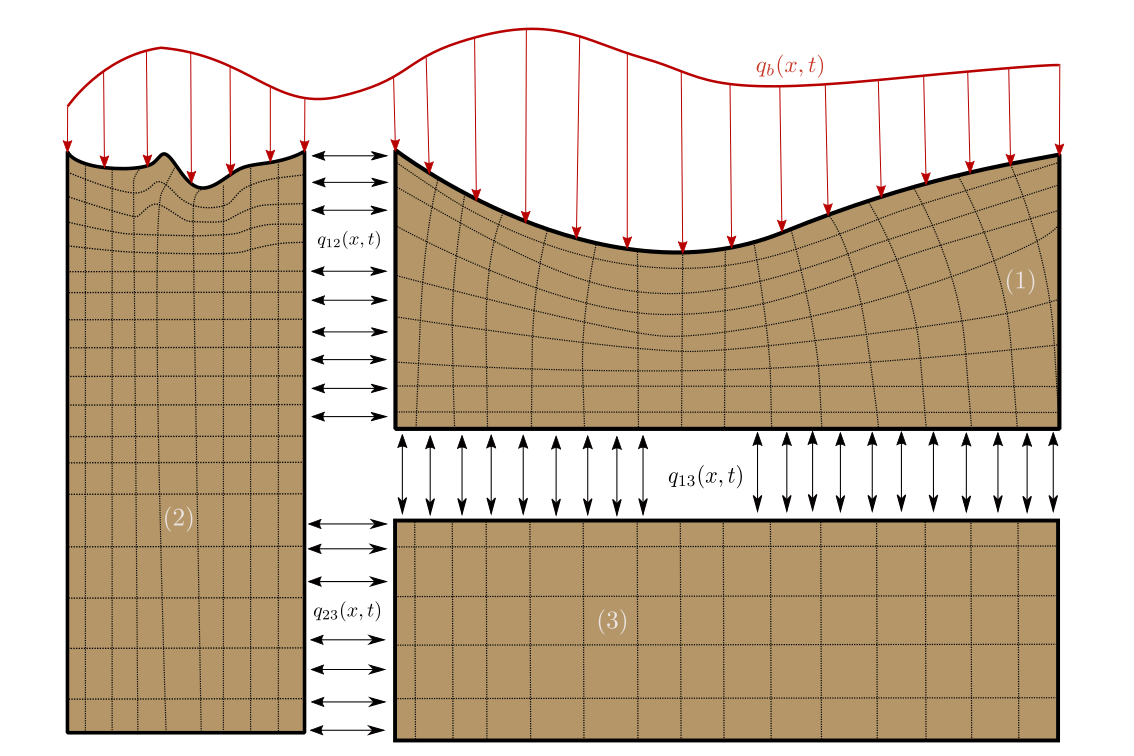
\includegraphics[width=0.8\textwidth]{./figs/three_components.png}
    \caption{Partition of the TPS into three one-dimensional components.}
    \label{fig_domain_partition}
\end{figure}

A first-order FEM scheme is adopted for each component, which results in a block-diagonal system of ODEs for the nodal temperature values of the components,
\begin{equation}
    \vA\left(\bvu\right)\dot{\bvu} = \left(\vB + \vC(t)\right)\bvu + \vf\left(\bvu,t\right)\label{eqn_rpm}
\end{equation}
where the block matrices are defined as,
\begin{subequations}
\begin{align}
\begin{aligned}
    \vA_{ij} &= \begin{cases}
        \vA^{(i)}(\bvu^{(i)}), & i=j \\
        0, & i\neq j
    \end{cases}\\
    \vB_{ij} &= \begin{cases}
        \vB^{(i)}(\bvu^{(i)}), & i=j \\
        0, & i\neq j
    \end{cases}
\end{aligned}
&\qquad
\begin{aligned}
    \vC_{ij}(t) &= \begin{cases}
        \vC^{(i)}(t), & i=j \\
        0, & i\neq j
    \end{cases}\\
    \mathbf{f}_i(\bvu,t) &= \begin{cases}
        \mathbf{f}^{(i)}_{\text{BC}}(t)+\mathbf{f}^{(i)}_{\cQ}(\bvu,t), & i=j \\
        \boldsymbol{0}, & i\neq j
    \end{cases}
\end{aligned}\label{eqn_rpm_matrices}
\end{align}
\end{subequations}
where $\vfBC$ and $\vfQ$ are the boundary and component-level energy sources. 


\subsubsection{Coarse Graining}

Consider a DG model as in ~\cref{eqn_energy_fem} for $M$ components and $N$ elements; clearly $N\gg N$. Let $\cV_j=\left\{i | E^{(i)}\in\Omega^{(j)}\right\}$ be the indices of the elements belonging to the $j$-th component, so $E^{(i)}\in\Omega^{(j)}$ for $i\in\cV_j$; number of elements in $\Omega^{(j)}$ is denoted as $\left|\cV_j\right|$.



The ablation on the $i$-th component is modeled using a one-dimensional approximation to the temperature and mesh-motion equations in \cref{eqn_governing_equations}, and are given by,
\begin{subequations}
    \begin{align}
        \rho c_p\left(\frac{\partial T^{(i)}}{\partial t} - v^{(i)}(x,t)\frac{\partial T^{(i)}}{\partial x}\right) - \frac{\partial}{\partial x}\left(k\frac{\partial T^{(i)}}{\partial x}\right) - \cQ^{(i)}_{\text{net}}(x,t) &= 0\label{eqn_thermal_1d}\\
        \frac{\partial}{\partial x}\left(\frac{\partial u^{(i)}}{\partial x}\right) &= 0\label{eqn_elasticity_1d}
    \end{align}\label{eqn_rpm}
\end{subequations}
with boundary conditions for the energy equation,
\begin{subequations}
    \begin{align}
        -k\frac{\partial T^{(i)}}{\partial x}\Bigg|_{x=0} &= q^{(i)}_b(t)\\
        -k\frac{\partial T^{(i)}}{\partial x}\Bigg|_{x=\ell} &= 0
    \end{align}
\end{subequations}
and for the elasticity equation,
\begin{subequations}
    \begin{align}
        u^{(i)}(0,t) &= \int_{t_0}^{t}v^{(i)}(\tau)d\tau = \int_{0}^{t} f(T^{(i)}_w(\tau))d\tau\\
        u^{(i)}(\ell,t) &= 0
    \end{align}
\end{subequations}
where $v^{(i)}(t)$ is the surface receding velocity due to ablation, which is a function of the surface temperature as in \cref{eqn_boundary_displacement}. The surface velocity is computed from a cubic spline interpolate to a B' look-up table...



\subsubsection{Thermal Solver}

The FEM implementation details are supplied in Appendix~\hl{x}. For the $n$-th component, the result of the FEM discretization is a system of ODEs for the nodal temperatures, coupled to the neighboring component $n+1$ through the energy volumetric source term,
\begin{equation}
    \mathbf{A}^{(i)}\frac{d\mathbf{T}^{(i)}}{dt} + \left(\mathbf{B}^{(i)} - \mathbf{C}^{(i)}(t)\right)\mathbf{T}^{(i)} = \mathbf{f}^{(i)}(t)
\end{equation}
where,
\begin{itemize}
    \item $\mathbf{A}^{(i)}\in\mathbb{R}^{M\times M}$ is the mass matrix,
    \item $\mathbf{B}^{(i)}\in\mathbb{R}^{M\times M}$ is the stiffness matrix,
    \item $\mathbf{C}^{(i)}(t)\in\mathbb{R}^{M\times M}$ is the advection matrix,,
    \item $\mathbf{T}^{(i)}\in\mathbb{R}^{M}$ is the vector of nodal temperatures, and
    \item $\mathbf{f}^{(i)}(t)\in\mathbb{R}^{M}$ is the input vector, which includes the Neumann boundary conditions and the net volumetric energy source term $\cQ^{(i)}_{\text{net}}$.
\end{itemize}
where $M$ is the number of nodes in the one-dimensional mesh for the $i$-th component.

\subsubsection{Pseudo-Elastic Solver}

Note that \cref{eqn_elasticity_1d} is steady. Under the assumption that the mesh deformation is quasi-steady, it can be applied at each time step within an ablation simulation. For instance, a known value of the wall temperature $T_w(t)$ specifies a Dirichlet boundary condition for the displacement, and the resulting nodal displacements within the ablator are determined from \cref{eqn_elasticity_pde}.

Along the one-dimensional domain, the PDE in \cref{eqn_elasticity_pde} simplifies to,
\begin{equation}
    \frac{\partial^2 u^{(i)}}{\partial x^2} = 0
\end{equation}
which has the analytical solution,
\begin{equation}
    u^{(i)}(x,t) = a(t)x + b(t)
\end{equation}
Imposing the boundary conditions leads to,
\begin{equation}
    u^{(i)}(x,t) = u^{(i)}(0,t)\left(\frac{x_1^{(i)} - x}{h^{(i)}}\right)
\end{equation}
The mesh velocity is the time derivative of the displacement,
\begin{equation}
    v^{(i)}(x,t) = \frac{\partial u^{(i)}(x,t)}{\partial t} = v^{(i)}(t)\left(\frac{x_1^{(i)} - x}{h^{(i)}}\right)
\end{equation}

\subsubsection{Coupling Scheme}

\subsubsection{Reduced-Physics Ablation Simulation}








\section{Physics-Infused Reduced-Order Modeling}\label{sec_pirom}
The formulation of PIROM for ablating TPS starts by connecting the FOM, i.e., DG-FEM, and the RPM, i.e., the LCM, via a coarse-graining procedure. This procedure pinpoints the missing dynamics in the LCM when compared to DG-FEM. Subsequently, the Mori-Zwanzig (MZ) formalism is employed to determine the model form for the missing dynamics in PIROM. Lastly, the data-driven identification of the missing dynanmics in PIROM is presented.

\subsection{Deriving the Reduced-Physics Model via Coarse-Graining}
The LCM is derived from a full-order DG on a fine mesh via a projection process, i.e., coarse graining. This process constraints the trial function space of a full-order DF model to a subset of piece-wise constants, so that the variables $\vu$, matrices $\vA$, $\vB$, and $\vC$, and forcing vector $\vf$ are all approximated using a single state associated to the average temperature. The details of the projection are described next.

\subsubsection{Coarse-Graining of States}

Consider a DG model as in \cref{eqn_full_dg} for M elements and an LCM as in \cref{eqn_lcm} for $N$ components; clearly $M\gg N$. 


\newpage\appendix
\section{Technical Details}\label{appendix}

This appendix presents the technical details of the PIROM framework applied to the TPS ablation problem. The first section provides the mathematical details for the definition of the DG-FEM. The second section follows the projection procedures from Ref.\hl{x}, and demonstrates the effects of coarse-graining on the advection matrix. The third section presents the derivation of the LCM model from an energy-conservation perspective.

\subsection{Full-Order Model}

To obtain the full-order numerical solution, the governing equation is spatially discretized using variational principles of Discontinuous Galerkin (DG) to result in a high-dimensional system of ordinary differential equations (ODEs). The DG-FEM model is written in an element-wise form, which is beneficial for subsequent derivations of the lower-order models.Note that the choice of DG approach here is mainly for theoretical convenience in the subsequent coarse-graining formulation. In the numerical results, the full-order TPS ablation simulations is computed using standard FEM instead, and the equivalence between DG and standard FEM is noted upon their convergence.

\subsubsection{Domain Discretization}

Consider a conforming mesh partition of the domain, as shown in Fig.\hl{DOMAIN}, where each element belongs to one and only one component. Denote the collection of all $M$ elements as $\left\{E_i\right\}_{i=1}^{M}$. To ease the description of the DG model, a graph structure is employed. The elements are treated as vertices, the set of which is denoted $\cV=\left\{m\right\}_{m=1}^{M}$. Two neighboring elements, $E_i$ and $E_j$, are connected by an edge $(i,j)$, and the shared boundary between them is denoted $\eij$. The collection of all edges are denoted $\cE$, and $\cG$ is referred to as a graph. In the graph, the edges are unidirected, meaning if $(i,j)\in\cE$ then $(j,i)\in\cE$. Furthermore, denote the neighbors of the $i$-th element as $\cN_i=\left\{j | (i,j) \in\cE\right\}$. Lastly, for the ease of notation, introduce two special indices: $T$ for the boundary of an element that overlaps with the Dirichlet boundary condition, and similarly $q$ for the Neumann boundary condition.

\subsubsection{Weak Form of Discontinuous Galerkin Method}

Choosing appropriate basis functions $\phi_k$ and $\phi_l$ and using the Interior Penalty Galerkin (IPG) scheme ~\cite{Cohen and pernet 2018}, the variational bilinear form for \cref{eqn_thermal_pde} is,
\begin{equation}
    \sum_{i=1}^{M}a_{\epsilon,i}(\phi_k,\phi_l) = \sum_{i=1}^{M}L_i(\phi_k)
\end{equation}
where $\epsilon$ is an user-specified parameter and,
\begin{subequations}
    \begin{align}
        a_{\epsilon,i}(\phi_k,\phi_l) &= \int_{E^{(i)}}\left(\rho c_p \phik \frac{\partial \phil}{\partial t} + \nabla \phik\cdot\left(\mathbf{k}\nabla \phil\right) - \rho c_p \phik \vv\cdot\nabla\phil\right)dE^{(i)}\\
        &= -\sum_{j\in\cN_i\cup\dirichletset}\int_{\eij}\average{\bk\nabla\phik\cdot n}\jump{\phil}d\eij + \epsilon\sum_{j\in\cN_i\cup\dirichletset}\int_{\eij}\average{\bk\nabla\phil\cdot n}\jump{\phik}d\eij \notag\\
        &+ \sigma\sumneighbordirichlet\int_{\eij}\jump{\phik}\jump{\phil}d\eij\\
        L_i(v) &= \epsilon\sumneighbordirichlet\int_{\eij}\left(\bk\nabla\phil\cdot n\right)T_b d\eij + \int_{\eiq}\phik q_b d\eiq + \sigma\int_{\eiT}\phik T_b d\eiT
    \end{align}
\end{subequations}
In the bi-linear form above, the notations $\jump{}$ and $\average{}$ are respectively the jumps and averages at the boundary $\eij$ share by two elements $E_i$ and $E_j$,
\[
    \jump{u} = u\big|_{E_i} - u\big|_{E_j},\quad \average{u} = \frac{1}{2}\left(u\big|_{E_i} + u\big|_{E_j}\right), \quad \text{for } x\in\eij = E_i\cap E_j
\]
Furthermore, in the bi-linear form, the terms associated with $\sigma$ are introduced to enforce the Dirichlet boundary conditions; $\sigma$ is a penalty factor whose value can depend on the size of an element. Depending on the choice of $\epsilon$, the bi-linear form corresponds to symmetric IPG ($\epsilon=-1$), non-symmetric IPG ($\epsilon=1$), and incomplete IPG ($\epsilon=0$). All these schemes are consistent with the original PDE and have similar convergence rate with respect to mesh size. In the following derivations, the case $\epsilon=0$ is chosen for the sake of simplicity.

\subsubsection{Discontinuous Galerkin Model}

Next, the DG-based model is written in an element-wise form. For the $i$-th element, use a set of $P$ trial functions to represent the temperature as in \cref{eqn_element_temperature}. Without loss of generality, the trial functions are assumed to be orthogonal, so that $\int_{E^{(i)}} \phii_k(x) \phii_l(x) dx = \left|\Ei\right|\delta_{kl}$, where $\left|\Ei\right|$ is the area $(n_d=2)$ or volume $(n_d=3)$ of the $i$-th element, and $\delta_{kl}$ is the Kronecker delta.

Using test functions same as trial functions, the dynamics $\vu^{(i)}$ is obtained by evaluating the element-wise bi-linear forms,
\begin{equation}
    a_{\epsilon,i}(\phik^{(i)},T^{(i)}) = L_i(\phik^{(i)}),\quad k=1,2,\dots,P
\end{equation}
The above procedure yields,
\begin{equation}
    \vA^{(i)}\dot{\vu}^{(i)} = \left(\vB^{(i)} + \vC^{(i)}(t)\right)\vui + \sumneighbordirichlet\left(\vB^{(i)}_{ij}\vui + \vB^{(j)}_{ij}\vuj\right) + \vf^{(i)}(t)\label{eqn_element_wise_model}
\end{equation}
where for $k,l=1,2,\dots,P$,
\begin{subequations}
    \begin{align}
        \left[\vA^{(i)}\right]_{kl} &= \intEi\rho c_p\phik^{(i)}\phil^{(i)}d\Ei\\
        \left[\vB^{(i)}\right]_{kl} &= -\intEi\left(\nabla\phik^{(i)}\right)\cdot\left(\vk\nabla\phil^{(i)}\right)d\Ei\\
        \left[\vC^{(i)}\right]_{kl} &= \intEi\rho c_p \phik^{(i)}\vv^{(i)}\cdot\nabla\phil^{(i)}d\Ei\\
        \left[\vBi_{ij}\right] &= \int_{\eij}\average{\vk\nabla\phik^{(i)}\cdot\hat{n}}\phil^{(i)} - \sigma\jump{\phik^{(i)}}\phil^{(i)}d\eij\\
        \left[\vBj_{ij}\right] &= \int_{\eij}-\average{\vk\nabla\phik^{(i)}\cdot\hat{n}}\phil^{(j)} + \sigma\jump{\phik^{(i)}}\phil^{(j)}d\eij\\
        \left[\vf^{(i)}\right]_k &= \int_{\eiq}\phik^{(i)}q_bd\eiq + \sigma\int_{\eiT}\phik^{(i)}d\eiT
    \end{align}
\end{subequations}
The matrices $\vA^{(i)}\in\mathbb{R}^{P\times P}$, $\vB^{(i)}\in\mathbb{R}^{P\times P}$, and $\vC^{(i)}\in\mathbb{R}^{P\times P}$ are respectively the capacitance, conductivity, and advection matrices for element $i$. These matrices depend on $\rho$, $c_p$, and $\vk$, and hence can be non-linear functions of $\vu^{(i)}$. Since the trial functions are orthogonal, if $\rho c_p$ is constant within an element, $\vAi$ is diagonal; otherwise, $\vA_i$ is symmetric and positive definite as $\rho c_p > 0$.

For compactness, the element-wise model in \cref{eqn_element_wise_model} is also written in matrix form,
\begin{equation}
    \vA(\dot{\vu}) = \left[\vB(\vu) + \vC(t,\vu)\right]\vu + \mathbf{f}(t)\label{eqn_complete_model}
\end{equation}
where $\vu = \left[\vu^{(1)},\vu^{(2)},\cdots,\vu^{(M)}\right]^T\in\mathbb{R}^{MP}$ includes all DG variables, $\vf=\left[\vf^{(1)},\vf^{(2)},\dots,\vf^{(M)}\right]^T\in\mathbb{R}^{MP}$, $\vA$ and $\vC$ are matrices of $M$ diagonal blocks whose $i$-th blocks are $\vAi$ and $\vCi$, and $\vB$ is a matrix of $M\times M$ blocks whose $(i,j)$-th block is,
\begin{equation}
    \vB_{ij} = \begin{cases}
            \vBi + \sumneighbordirichlet\vBi_{ij}, & i=j\\
            \vBj_{ij}, & i\neq j
        \end{cases}
\end{equation}
The dependency of $\vA$, $\vB$, and $\vC$ on $\vu$ is explicitly noted in \cref{eqn_complete_model}, which is the source of non-linearity in the current TPS problem. Moreover, the mesh velocity $\vv$ varies with space and time, and thus the advection matrix $\vC$ varies with time as a function of $q_b$.

\subsection{Coarse-Graining of Dynamics}

The LCM is obtained by coarse-graining the full-order DG-FEM. This coarse-graining procedure produces resolved $\vr^{(1)}(\vu,t)$ and residual $\vr^{(2)}(\vu,t)$ dynamics as in \cref{eqn_coarse_grained_dynamics}. This section presents the detail derivations and magnitude analysis for the resolved and residual dynamics.

\subsubsection{Resolved Dynamics}

Using \cref{eqn_projection_operator}, the resolved dynamics is computed as follows,
\begin{subequations}
    \begin{align}
        &\vr^{(1)}(\vu,t) = \cP\left[\vPhiplus\vA(\vu)^{-1}\left(\vB(\vu)\vu + \vC(t,\vu)\vu + \vf(t,\vu)\right)\right]\\
        &= \vPhiplus\vA\left(\vP\vu\right)^{-1}\vP\vB\left(\vP\vu\right)\vP\vu + \vPhiplus\vA\left(\vP\vu\right)^{-1}\vP\vC\left(t,\vP\vu\right)\vP\vu + \vPhiplus\vA\left(\vP\vu\right)^{-1}\vP\vf(t,\vP\vu)\\
        &= \underbrace{\vPhiplus\vA\left(\vPhi\bvu\right)^{-1}\vPhi}_{\text{\#1}}\underbrace{\vPhiplus\vB\left(\vPhi\bvu\right)\vPhi\bvu}_{\text{\#2}} + \vPhiplus\vA\left(\vPhi\bvu\right)^{-1}\vPhi\underbrace{\vPhiplus\vC\left(t,\vPhi\bvu\right)\vPhi}_{\text{\#3}}\bvu + \vPhiplus\vA\left(\vPhi\bvu\right)^{-1}\vPhi\underbrace{\vPhiplus\vf(t,\vPhi\bvu)}_{\text{\#4}}
    \end{align}
\end{subequations}
Detailed derivations for the \#1, \#2, and \#4 terms can be found in Ref.\hl{x}. The effects of coarse-graining on term \#3 are analyzed next.

The $\vC(t,\vu)\in\mathbb{R}^{MP\times MP}$ matrix is block diagonal, since the basis functions are defined locally on each element, therefore, $\left[\vC(t,\vu)\right]_{ij} = \vzero$ for all $i \neq j$. Moreover, since the first basis function is constant, $\nabla\phi_1^{(i)} = 0$ and thus the first row and first column of each block $\vCi$ are zero. It follows that for $k,l=1,2,\cdots,N$,
\begin{subequations}
    \begin{align}
        \left[\vPhiplus\vC(t,\vPhi\bvu)\vPhi\right]_{kl} &= \sum_{i=1}^{M}\sum_{j=1}^{M}\vvarphi_{i}^{k+}\left[\vC(t,\vPhi\bvu)\right]_{ij}\vvarphi_{j}^{l}\\
        &= \sum_{i=1}^{M}\vvarphi_{i}^{k+}\left[\vC(t,\vPhi\bvu)\right]_{ii}\vvarphi_{i}^{l}\\
        &= 
    \end{align}
\end{subequations}


\subsubsection{Magnitude Analysis for Residual Dynamics}

\subsection{Lumped Capacitance Model}

The following assumptions are employed: (1) the temperature in component $(i)$ is described by a scalar time-varying average temperature $\bar{u}^{(i)}$, (2) between neighboring components $(i)$ and $(j)$ the heat flux is approximated as,
\begin{equation}
    q_{ij} = \frac{\baruj - \barui}{R_{ij}}
\end{equation}
where $R_{ij}$ is the thermal resistance. Empirically, for a component of isotropic heat conductivity $k$, length $\ell$, and cross-section area $A$, the thermal resistance is $R=\ell/kA$. Between components $i$ and $j$, define $R_{ij}=R_{i} + R_{j}$. In addition, the heat flux due to Dirichlet boundary condition is computed as $q_{iT} = (T_b - \barui)/R_{i}$.

At component $i$, the dynamics of LCM are given by,
\begin{subequations}
    \begin{align}
        \int_{\Ei}\rho c_p \dot{\bar{u}}^{(i)} d\Ei &= \left(\sumneighbori\int_{\eij}\frac{\baruj - \barui}{R_{ij}}d\eij\right) + \int_{\eiq} q_b d\eiq + \int_{\eiT}\frac{T_b - \barui}{R_i}d\eiT\label{eqn_lcm_1}\\
        \bar{A}^{(i)}\dot{\bar{u}}^{(i)} &= \left(\sumneighbori\frac{|\eij|}{R_{ij}}\left(\baruj - \barui\right)\right) + |\eiq|\bar{q}^{(i)} + \frac{|\eiT|}{R_i}\left(\bar{T}^{(i)} - \barui\right) \label{eqn_lcm_2}\\ 
        &= \sumneighbori\left(-\frac{|\eij|}{R_{ij}}\barui + \frac{|\eij|}{R_{ij}}\baruj\right) + \left(-\frac{|\eiT|}{R_{i}}\barui\right) + \left(|\eiq|\bar{q}^{(i)} + \frac{|\eiT|}{R_i}\bar{T}^{(i)}\right)\label{eqn_lcm_3}\\
        &= \sumneighbordirichlet\left(\bar{B}^{(i)}_{ij}\barui + \bar{B}^{(j)}_{ij}\baruj\right) + \bar{f}^{(i)}\label{eqn_lcm_4}
    \end{align}
\end{subequations}
where in \cref{eqn_lcm_2} $|e|$ denotes the length $(d=2)$ or area $(d=3)$ of a component boundary $e$. The $\bar{A}^{(i)}$, $\bar{B}_{ij}^{(i)}$, and $\bar{B}_{ij}^{(j)}$ quantities are provided in \cref{eqn_lcm_matrices_elements}.

The lumped-mass representation for the four-component TPS is shown in Fig.~\ref{fig_four_components}. Let $v_i$ represent the area of the $i$-th element, $\overline{\rho c_p}_{,i}$, the heat capacity evaluated using the average temperature $\bu^{(i)}$, and $1/R_{ij} = 1/R_{i}(\bu^{(i)}) + 1/R_{j}(\bu^{(j)})$ the equivalent thermal resistance between elements $i$ and $j$. Leveraging the formulas from \cref{eqn_lcm_matrices,eqn_lcm_matrices_elements}, the LCM matrices are given by,
\begin{subequations}
    \begin{gather}
        \bar{\vA} = \begin{bmatrix}
            \overline{\rho c_p}_{,1} v_1 & 0 & 0 & 0\\
            0 & \overline{\rho c_p}_{,2} v_2 & 0 & 0\\
            0 & 0 & \overline{\rho c_p}_{,3} v_3 & 0\\
            0 & 0 & 0 & \overline{\rho c_p}_{,4} v_4
        \end{bmatrix},\\
        \bar{\vB} = \begin{bmatrix}
            \frac{1}{R_{12}} + \frac{1}{R_{14}} & -\frac{1}{R_{12}} & 0 & -\frac{1}{R_{14}}\\
            -\frac{1}{R_{12}} & \frac{1}{R_{12}} + \frac{1}{R_{24}} + \frac{1}{R_{23}} & -\frac{1}{R_{23}} & -\frac{1}{R_{24}}\\
            0 & -\frac{1}{R_{32}} & \frac{1}{R_{32}} + \frac{1}{R_{34}} & -\frac{1}{R_{34}}\\
            -\frac{1}{R_{14}} & -\frac{1}{R_{24}} & -\frac{1}{R_{34}} & \frac{1}{R_{14}} + \frac{1}{R_{24}} + \frac{1}{R_{34}}
        \end{bmatrix},\quad \bar{\vf} = \begin{bmatrix}
            \bar{q}^{(1)} \\
            \bar{q}^{(2)} \\
            \bar{q}^{(3)} \\
            0
        \end{bmatrix}
    \end{gather}
\end{subequations}




\end{document}
